\documentclass[11pt]{beamer}
\usetheme{CambridgeUS}
\usepackage[utf8]{inputenc}
\usepackage{amsmath}
\usepackage{amsfonts}
\usepackage{amssymb}
\usepackage{graphicx}
\usepackage{pgfpages}
\usepackage{framed}
\usepackage{xcolor}
\usepackage[most]{tcolorbox}
\usepackage{soul}
\usepackage{empheq}
\usepackage{booktabs}
\usepackage{listings}

% The replacement character � (often displayed as a black rhombus with a white
% question mark) is a symbol found in the Unicode standard at code point U
% +FFFD in the Specials table. It is used to indicate problems when a system 
% is unable to render a stream of data to a correct symbol.[4] It is usually 
% seen when the data is invalid and does not match any character. For this 
% reason we map explicitly this character to a blanck space.
\DeclareUnicodeCharacter{FFFD}{ }

\newcommand*{\itemimg}[1]{%
  \raisebox{-.3\baselineskip}{%
    \includegraphics[
      height=\baselineskip,
      width=\baselineskip,
      keepaspectratio,
    ]{#1}%
  }%
}

\newtcbox{\mymath}[1][]{%
    nobeforeafter, math upper, tcbox raise base,
    enhanced, colframe=blue!30!black,
    colback=blue!10, boxrule=1pt,
    #1}

\newcommand{\highlight}[1]{%
  \colorbox{yellow!50}{$\displaystyle#1$}}

\author{Giovanni Della Lunga\\{\footnotesize giovanni.dellalunga@unibo.it}}
%\title{1.1 - Introduction to Machine Learning}
%\title{1.2 - Data Gathering with Pandas}
\title{2.2 - Feature Engineering and Dimensionality Reduction}
%\title{4.1 - Linear and Logistic Regression}
%\title{4.2 - Decision Trees}
%\title{6 - Text Vectorization}
%\title{7 - Classification for Text Analysis}
%\title{8 - Clustering for Text Similarity}
%\title{9 - Information Extraction}
\subtitle{} % (optional)
\setbeamercovered{transparent} 
\institute{Introduction to Machine Learning for Finance} 
\date{Bologna - February-March, 2025} 

\begin{document}

%\begin{frame}
%\includegraphics[width=\linewidth]{img/halloween-seminar-logo.PNG}
%\end{frame}

\begin{frame}
\titlepage
\end{frame}

\AtBeginSection[]
{
  %\begin{frame}<beamer>
  %\footnotesize	
  %\frametitle{Outline}
  %\begin{multicols}{2}
  %\tableofcontents[currentsection]
  %\end{multicols}	  
  %\normalsize
  %\end{frame}
  \begin{frame}
  \vfill
  \centering
  \begin{beamercolorbox}[sep=8pt,center,shadow=true,rounded=true]{title}  	\usebeamerfont{title}\insertsectionhead\par%
  \end{beamercolorbox}
  \vfill
  \end{frame}
}
\AtBeginSubsection{\frame{\subsectionpage}}
%
%---------------------------------------------------------------------------------------------------
%
\section{Feature Selection}
%
%---------------------------------------------------------------------------------------------------
%
\begin{frame}{Introduction to Feature Selection}
    \begin{itemize}
        \item Feature selection is the process of identifying and retaining only the most relevant variables for a machine learning model.
        \item The goal is to improve model performance by reducing noise and redundancy in the dataset.
        \item High-dimensional datasets often contain irrelevant or correlated features that do not contribute meaningful information for prediction.
        \item Unlike feature extraction, which transforms existing features into new ones (e.g., PCA, LDA), feature selection retains a subset of the original features.
        \item Feature selection enhances interpretability, reduces training time, and prevents overfitting, leading to a more efficient and effective model.
    \end{itemize}
\end{frame}
%
%..................................................................
%
\begin{frame}{Why Feature Selection is Important?}
    \begin{itemize}
        \item \textbf{Reduces Overfitting}: By removing irrelevant or redundant features, the model focuses only on meaningful variables, reducing the risk of learning noise instead of true patterns.
        \item \textbf{Improves Accuracy}: By eliminating uninformative features, the model generalizes better to unseen data, leading to improved prediction performance.
        \item \textbf{Speeds Up Training}: Fewer features mean lower computational complexity, reducing the time required to train and optimize machine learning models.
   \end{itemize}     
\end{frame}
%
%..................................................................
%
\begin{frame}{Why Feature Selection is Important?}
    \begin{itemize}
        \item \textbf{Enhances Interpretability}: Models with fewer, well-selected features are easier to understand and explain, which is especially important in regulated industries such as finance and healthcare.
        \item \textbf{Mitigates Curse of Dimensionality}: High-dimensional data can negatively impact model performance due to sparsity; selecting relevant features helps mitigate this issue.
        \item \textbf{Facilitates Model Deployment}: A model with fewer variables is easier to implement in production environments, requiring less storage and computational resources.
    \end{itemize}
\end{frame}
%
%..................................................................
%
\begin{frame}{How do we select features? }
	\begin{itemize}
		\item A feature selection procedure combines a search technique with an evaluation method. The search technique proposes new feature subsets, and the evaluation measure determines the how good the subset is.
		\item In a perfect world, a feature selection method would evaluate all possible subsets of feature combinations and determine which one results in the best performing machine learning model.
		\item However, computational cost inhibits such a practice in reality. In addition, the optimal subset of features varies between machine learning models. A feature subset that optimizes one model`s performance won`t necessarily optimize another`s.
	\end{itemize}
\end{frame}
%
%..................................................................
%
\begin{frame}{Methods of Feature Selection}
    \begin{enumerate}
        \item \textbf{Filter Methods}: These methods apply statistical techniques to evaluate the importance of each feature independently of the model. Common techniques include correlation analysis, Chi-square test, and mutual information.
        \item \textbf{Wrapper Methods}: These methods iteratively evaluate subsets of features using machine learning models, selecting the best-performing combination. Examples include Recursive Feature Elimination (RFE), Forward Selection, and Backward Elimination.
        \item \textbf{Embedded Methods}: These methods integrate feature selection within the model training process. Techniques such as Lasso (L1) regression and Decision Tree-based feature importance are commonly used.
    \end{enumerate}
\end{frame}
%
%..................................................................
%
\begin{frame}{Filter Methods}
	\begin{itemize}
		\item A typical filter algorithm consists of two steps: it ranks features based on certain criteria and then chooses the highest-ranking features to train the machine learning models.
		\item Filter methods are generally univariate, so they rank each feature independently of the rest. Because of this, the filter methods tend to ignore any interactions that occur between features. Thus, redundant variables will not necessarily be eliminated by filter methods.
		\item However, some multivariate filter selection methods exist as well. These consider features in relations to others in the data set, making them naturally capable of handling redundant features. Their selection criteria scans for duplicated features and correlated features and provide simple but powerful methods to quickly remove redundant information.
	\end{itemize}
\end{frame}
%
%..................................................................
%
\begin{frame}{Filter Methods}
\textbf{Constant, quasi-constant, and duplicated features}
	\begin{itemize}
		\item The most basic and intuitive methods for feature selection consist of removing constant, quasi-constant, or duplicated features.
		\item Constant features only show one value for all the observations in the data set. That is, they show absolutely no variability.
		\item Quasi-constant features are similar; if most observations share the same value, then we`d label that feature quasi-constant. In practice, quasi-constant features typically refer to those variables where more than 95 to 99 percent of the observations show the same value.
		\item Duplicated features, as the name indicates, are those that are in essence, identical. That is, for every observation, they show the same value.
	\end{itemize}
\end{frame}
%
%..................................................................
%
\begin{frame}{Filter Methods}
\textbf{Constant, quasi-constant, and duplicated features}
	\begin{itemize}
		\item Although it sounds obvious and overly simple, many datasets contain a lot of constant, quasi-constant, and duplicated features. 
		\item In fact, duplicated features often arise when generating new features by one-hot encoding of categorical variables. 
		\item Removing these features is an easy but effective way to reduce the dimension of the feature space, without losing any significant information.
	\end{itemize}
\end{frame}
%
%..................................................................
%
\begin{frame}{Filter Methods}
\textbf{Correlation}
	\begin{itemize}
		\item Correlation measures the linear association between two or more variables. 
		\item The higher the correlation, the more linearly associated the variables are. 
		\item The central hypothesis is that good feature sets contain features that are highly correlated with the target, yet uncorrelated with each other.
		\item If two variables are correlated, we can predict one from the other. 
		\item Therefore, if two features are correlated, the model only really needs one of them, as the second one does not add additional information.
	\end{itemize}
\end{frame}
%
%..................................................................
%
\begin{frame}{Filter Methods}
\textbf{Mutual Information}
	\begin{itemize}
		\item Mutual information measures the mutual dependence between two variables, in this case, the feature and the target. Mutual information is similar to correlation, but more general; it doesn`t strictly represent linear association. It measures how much knowing one of these variables reduces uncertainty in the other.
	\end{itemize}
\textbf{Fisher Score}
	\begin{itemize}
		\item Fisher score uses the Chi-Square distribution to measure the dependency between two variables and works with categorical or discrete variables.
		\item Fisher score essentially compares the actual frequencies of the values of a variable with the expected frequencies if it had no relation to the target.
	\end{itemize}
\end{frame}
%
%..................................................................
%
\begin{frame}{Wrapper Methods}
	\begin{itemize}
		\item \footnotesize{In comparison to filter methods, wrapper methods tend to be more computationally expensive, but select a better set of features.
		\item Wrapper methods use a specific machine learning algorithm in the selection process and choose the best subset of features tailored for that algorithm. 
		\item This subset of features may not be optimal for a different machine learning model. In other words, \textbf{wrapper methods are not model agnostic}.}
	\end{itemize}
	\begin{center}
	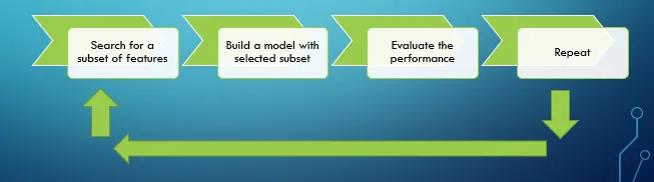
\includegraphics[scale=0.65]{../05-pictures/lesson-2-2_pic_4.png}
	\end{center}
\end{frame}
%
%..................................................................
%
\begin{frame}[fragile]{Example: RFE with Logistic Regression}{Wrapper Methods}
    \begin{lstlisting}[language=Python]
from sklearn.feature_selection import RFE
from sklearn.linear_model import LogisticRegression

model = LogisticRegression()
rfe = RFE(model, n_features_to_select=5)
rfe.fit(X_train, y_train)
selected_features = X_train.columns[rfe.support_]
print("Selected Features:", selected_features)
    \end{lstlisting}
\end{frame}
%
%..................................................................
%
\begin{frame}{Embedded Methods}
    \begin{itemize}
        \item Feature selection occurs during model training.
        \item Uses model-specific techniques.
        \item Examples:
        \begin{itemize}
            \item Lasso (L1) Regression
            \item Decision Trees and Random Forests
        \end{itemize}
    \end{itemize}
\end{frame}
%
%..................................................................
%
\begin{frame}{Comparison of Methods}
\center{
    \begin{tabular}{lcc}
        \toprule
        Method & Pros & Cons \\
        \midrule
        Filter & Fast, scalable & Ignores interactions \\
        Wrapper & Better selection & Expensive \\
        Embedded & Model-optimized & Model-dependent \\
        \bottomrule
    \end{tabular}
    }
\end{frame}
%
%..................................................................
%
\begin{frame}{Understanding Pipelines in Scikit-Learn}
    \begin{itemize}
        \item A pipeline is a sequence of data processing steps that are applied in a structured way.
        \item It helps automate machine learning workflows by chaining together multiple operations.
        \item Instead of manually applying transformations (e.g., scaling, feature selection, model training), a pipeline does it all in one step.
        \item Think of a pipeline as an assembly line: 
        \begin{itemize}
            \item Raw data enters the pipeline.
            \item The data is preprocessed (e.g., missing values handled, scaling applied).
            \item Feature selection picks the most relevant features.
            \item A machine learning model is trained on the transformed data.
            \item Predictions are generated efficiently.
        \end{itemize}
    \end{itemize}
\end{frame}
%
%..................................................................
%
\begin{frame}{Feature Selection Pipeline in Scikit-Learn}
    \begin{itemize}
        \item Machine learning pipelines in Scikit-Learn allow seamless integration of preprocessing, feature selection, and model training.
        \item They enhance workflow efficiency, reproducibility, and ensure that transformations are applied consistently during training and inference.
        \item A typical pipeline consists of:
        \begin{itemize}
            \item Preprocessing (e.g., standardization, encoding categorical variables)
            \item Feature Selection (e.g., Recursive Feature Elimination, SelectKBest)
            \item Model Training (e.g., Logistic Regression, Random Forest)
        \end{itemize}
        \item Pipelines prevent data leakage by ensuring that feature selection and scaling are only learned from the training data.
    \end{itemize}
\end{frame}
%
%..................................................................
%
\begin{frame}[fragile]{Example: Feature Selection Pipeline in Scikit-Learn}
\footnotesize{
    \begin{lstlisting}[language=Python]
from sklearn.pipeline import Pipeline
from sklearn.preprocessing import StandardScaler
from sklearn.feature_selection import SelectKBest, f_classif
from sklearn.linear_model import LogisticRegression

# Define the pipeline
pipeline = Pipeline([
# Standardize features
('scaler', StandardScaler()),  
# Select top 5 features
('feature_selection', SelectKBest(score_func=f_classif, k=5)), 
# Train logistic regression model 
('classifier', LogisticRegression()) 
])
# Fit the pipeline on training data
pipeline.fit(X_train, y_train)    
y_pred = pipeline.predict(X_test) # Make predictions
    \end{lstlisting}
}
\end{frame}
%
%..................................................................
%
\begin{frame}{Advantages of Using Pipelines}
    \begin{itemize}
        \item \textbf{Automation:} Reduces manual steps and minimizes human errors.
        \item \textbf{Prevents Data Leakage:} Ensures feature selection and scaling are applied correctly.
        \item \textbf{Code Reusability:} Simplifies experimentation with different models and preprocessing techniques.
        \item \textbf{Hyperparameter Tuning:} Easily integrates with GridSearchCV and RandomizedSearchCV for optimizing parameters.
    \end{itemize}
\end{frame}
%
%..................................................................
%
\begin{frame}{Conclusion and Best Practices}
    \begin{itemize}
        \item Choose method based on dataset size and complexity.
        \item Filter methods for quick insights.
        \item Wrapper methods for optimal selection.
        \item Embedded methods for model-specific optimization.
        \item Always validate selected features.
    \end{itemize}
\end{frame}
%
%---------------------------------------------------------------------------------------------------
%
\section{Dimensionality Reduction}
%
%---------------------------------------------------------------------------------------------------
%
\begin{frame}{Feature Selection: Follow a KISS Approach!}
	\begin{itemize}
		\item As a dimensionality reduction technique, feature selection aims to choose a small subset of the relevant features from the original features by removing irrelevant, redundant, or noisy features. 
		\item Feature selection usually can lead to better learning performance, higher learning accuracy, lower computational cost, and better model interpretability.
		\item The problem is important, because a high number of features in a dataset, comparable to or higher than the number of samples, leads to model overfitting, which in turn leads to poor results on the validation datasets. 
		\item Additionally, constructing models from datasets with many features is more computationally demanding.
	\end{itemize}
\end{frame}
%
%..................................................................
%
\begin{frame}{Feature Extraction and Feature Selection}
	\begin{itemize}
		\item Even though feature extraction and feature selection processes share some overlap, often these terms are erroneously equated. 
		\item \textbf{Feature extraction} is the process of using domain knowledge to extract new variables from raw data that make machine learning algorithms work. 
		\item The \textbf{feature selection} process is based on selecting the most consistent, relevant, and non-redundant features.
		\item The feature selection process is based on selecting the most consistent, relevant, and non-redundant feature subset from feature vectors. 
		\item It is not only reduces training time and model complexity, but it eventually helps to \textbf{prevent overfitting}.
	\end{itemize}
\end{frame}
%
%..................................................................
%
\begin{frame}{Principal Component Analysis (PCA)}
    \begin{itemize}
        \item PCA is a widely used technique that transforms the original features into a new set of orthogonal components.
        \item The first few principal components retain the most variance in the data.
        \item Helps in reducing dimensionality while preserving important patterns.
        \item PCA works by:
        \begin{itemize}
            \item Standardizing the dataset.
            \item Computing the covariance matrix.
            \item Finding eigenvectors and eigenvalues.
            \item Selecting the top principal components.
            \item Transforming the data into the new feature space.
        \end{itemize}
        \item PCA is effective for noise reduction and visualization.
    \end{itemize}
\end{frame}
%
%..................................................................
%
\begin{frame}{Mathematics Behind PCA}
    \begin{itemize}
        \item Given a dataset with $n$ features, PCA computes the covariance matrix:
        \begin{equation}
        C = \frac{1}{n} X^T X
        \end{equation}
        \item The eigenvectors and eigenvalues of $C$ represent the principal components and their importance.
        \item The data is projected onto the top $k$ eigenvectors with the highest eigenvalues:
        \begin{equation}
        Z = X W
        \end{equation}
        where $W$ is the matrix of selected eigenvectors.
    \end{itemize}
\end{frame}
%
%..................................................................
%
\begin{frame}{Standardization and Gradient Descent}
	\begin{center}
	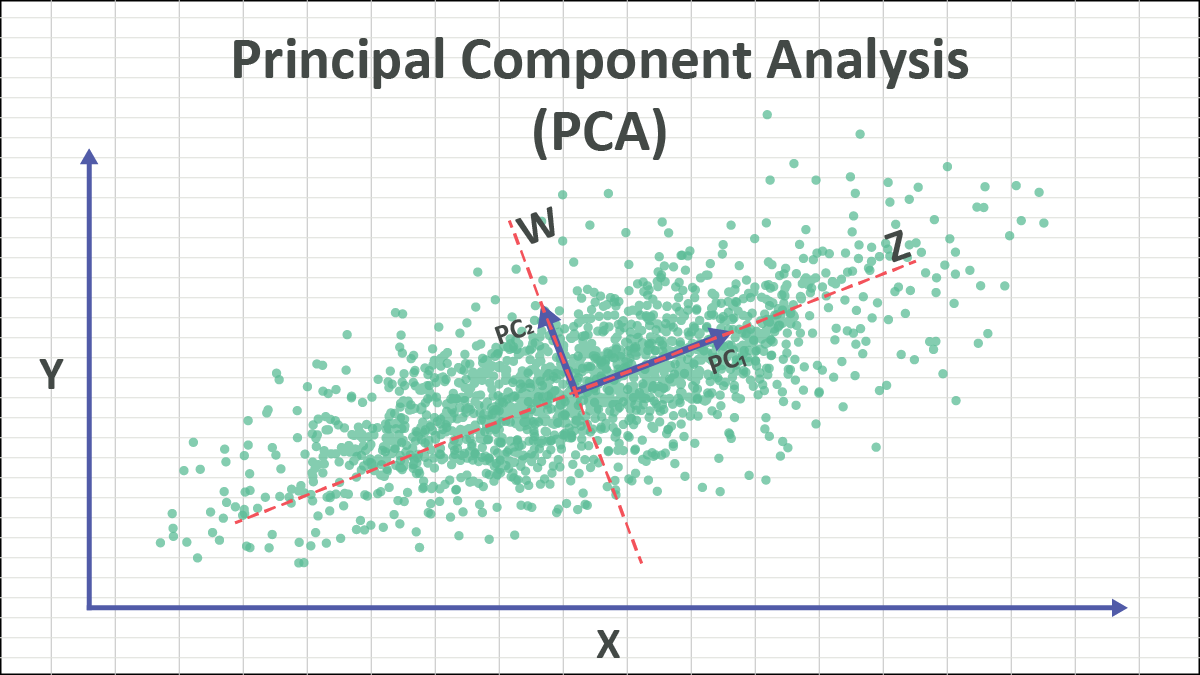
\includegraphics[scale=.375]{../05-pictures/lesson-2-2_pic_6.png}
	\end{center}
\end{frame}
%..................................................................
\begin{frame}[fragile]{Example: PCA in Scikit-Learn}
    \begin{lstlisting}[language=Python]
from sklearn.decomposition import PCA
from sklearn.preprocessing import StandardScaler

# Standardize the features
scaler = StandardScaler()
X_scaled = scaler.fit_transform(X)

# Apply PCA
pca = PCA(n_components=2)
X_pca = pca.fit_transform(X_scaled)
    \end{lstlisting}
\end{frame}
%
%..................................................................
%
\begin{frame}{Advantages and Limitations of PCA}
    \begin{itemize}
        \item \textbf{Advantages:}
        \begin{itemize}
            \item Reduces redundancy by removing correlated features.
            \item Improves model efficiency by reducing computation time.
            \item Helps in visualizing high-dimensional data.
        \end{itemize}
        \item \textbf{Limitations:}
        \begin{itemize}
            \item Assumes linear relationships in data.
            \item Loses interpretability of original features.
            \item Sensitive to data scaling; standardization is required.
        \end{itemize}
    \end{itemize}
\end{frame}
%
%..................................................................
%
\begin{frame}{When to Use PCA?}
    \begin{itemize}
        \item When dealing with high-dimensional data to reduce computational costs.
        \item When visualization of data is required in lower dimensions.
        \item When removing noise and redundancy is essential for better model performance.
        \item When feature interpretability is less important compared to efficiency.
    \end{itemize}
\end{frame}
%
%..................................................................
%
\begin{frame}{Linear Discriminant Analysis (LDA)}
    \begin{itemize}
        \item LDA is a supervised dimensionality reduction technique that maximizes class separability.
        \item Unlike PCA, which focuses on variance, LDA optimizes for class separation.
        \item Works well for classification problems by finding a lower-dimensional space that retains discriminative information.
        \item LDA assumes that different classes generate data based on Gaussian distributions with the same covariance matrix.
    \end{itemize}
\end{frame}
%
%..................................................................
%
\begin{frame}{LDA Vs PCA}
	\begin{center}
	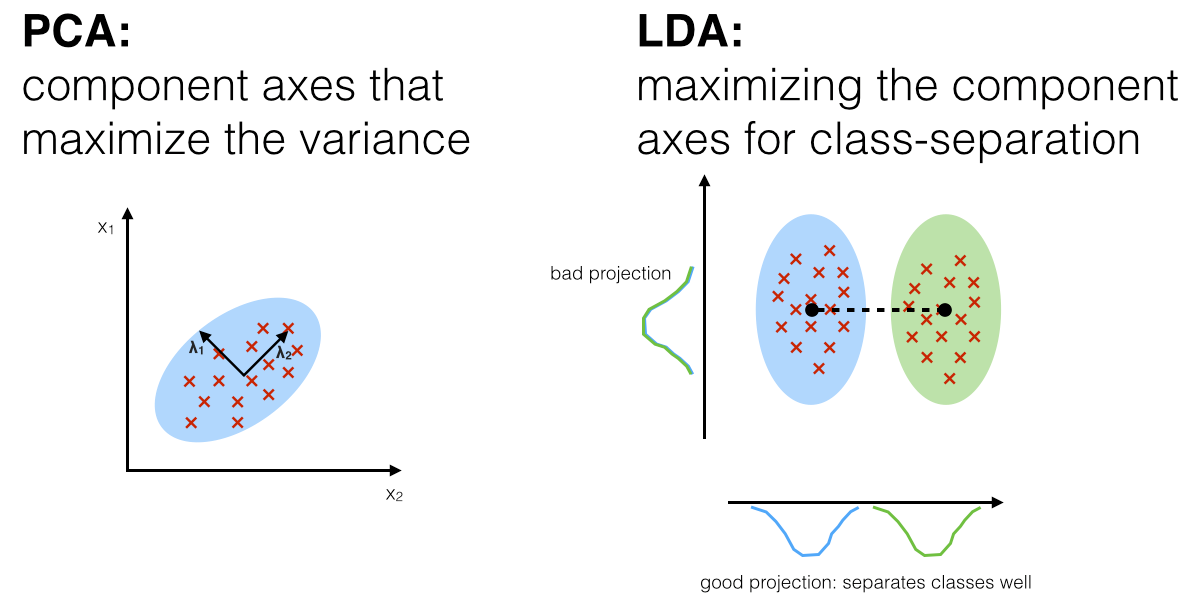
\includegraphics[scale=.375]{../05-pictures/lesson-2-2_pic_7.png}
	\end{center}
\end{frame}
%
%..................................................................
%
\begin{frame}{LDA Vs PCA}
	\begin{center}
	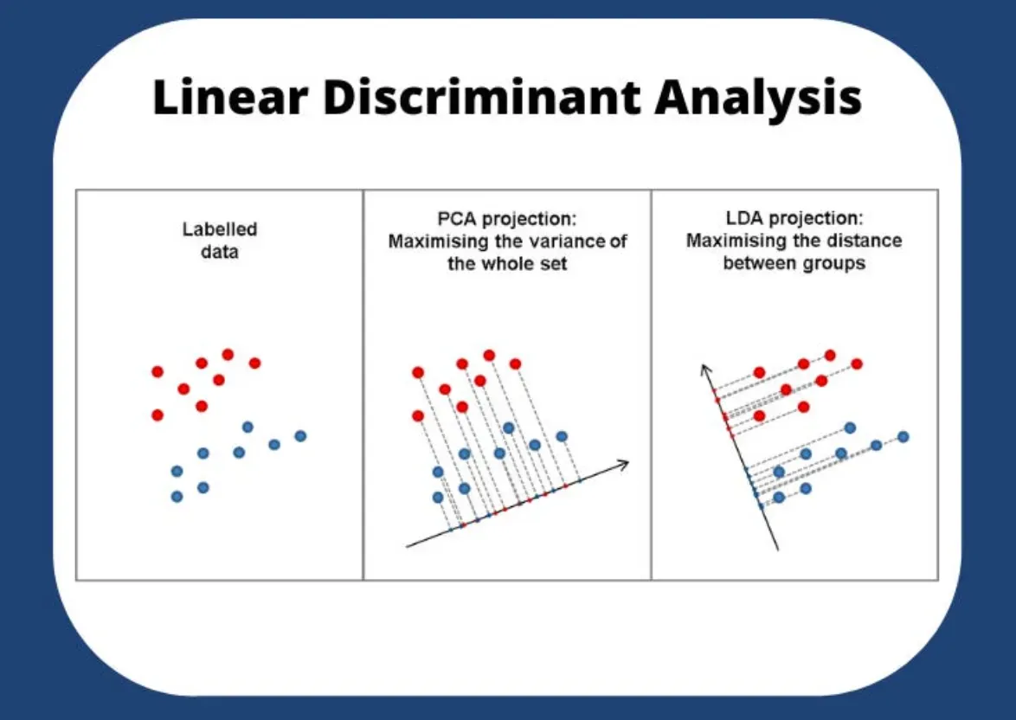
\includegraphics[scale=.375]{../05-pictures/lesson-2-2_pic_8.png}
	\end{center}
\end{frame}
%
%..................................................................
%
\begin{frame}{Mathematics Behind LDA}
    \begin{itemize}
        \item LDA computes two key matrices:
        \begin{itemize}
            \item Within-class scatter matrix ($S_W$): Measures variance within each class.
            \item Between-class scatter matrix ($S_B$): Measures variance between different classes.
        \end{itemize}
        \item LDA solves the generalized eigenvalue problem:
        \begin{equation}
        S_W^{-1} S_B v = \lambda v
        \end{equation}
        where eigenvectors corresponding to the largest eigenvalues define the optimal projection space.
    \end{itemize}
\end{frame}
%
%..................................................................
%
\begin{frame}[fragile]{Example: LDA in Scikit-Learn}
    \begin{lstlisting}[language=Python]
from sklearn.discriminant_analysis 
     import LinearDiscriminantAnalysis
     
from sklearn.preprocessing import StandardScaler

# Standardize the features
scaler = StandardScaler()
X_scaled = scaler.fit_transform(X)

# Apply LDA
lda = LinearDiscriminantAnalysis(n_components=2)
X_lda = lda.fit_transform(X_scaled, y)
    \end{lstlisting}
\end{frame}
%
%..................................................................
%
\begin{frame}{Advantages and Limitations of LDA}
    \begin{itemize}
        \item \textbf{Advantages:}
        \begin{itemize}
            \item Improves class separability in classification problems.
            \item Reduces dimensionality while preserving discriminative information.
            \item Computationally efficient compared to other non-linear methods.
        \end{itemize}
        \item \textbf{Limitations:}
        \begin{itemize}
            \item Assumes normally distributed classes with equal covariance matrices.
            \item Less effective when class distributions overlap significantly.
            \item Requires labeled data for training.
        \end{itemize}
    \end{itemize}
\end{frame}
%
%..................................................................
%
\begin{frame}{When to Use LDA?}
    \begin{itemize}
        \item When working with classification tasks that require feature reduction.
        \item When the goal is to maximize class separation in lower-dimensional space.
        \item When the dataset follows Gaussian distribution assumptions.
    \end{itemize}
\end{frame}
%
%..................................................................
%
\begin{frame}{Comparison: PCA vs LDA}
\center{
    \begin{tabular}{lcc}
        \toprule
        Method & Objective & Type \\
        \midrule
        PCA & Maximize variance & Unsupervised \\
        LDA & Maximize class separability & Supervised \\
        \bottomrule
    \end{tabular}
}
\end{frame}
%
%..................................................................
%
\begin{frame}{Conclusion}{LDA}
    \begin{itemize}
        \item LDA is a powerful tool for supervised dimensionality reduction, particularly in classification tasks.
        \item It optimizes feature space for class separability, making it useful for many real-world applications.
        \item Choosing between PCA and LDA depends on the problem: use PCA for general structure preservation and LDA for class separability.
    \end{itemize}
\end{frame}
%=====================================================================
\end{document}
%=====================================================================

%..................................................................
\begin{frame}{Standardization and Gradient Descent}
	\begin{center}
	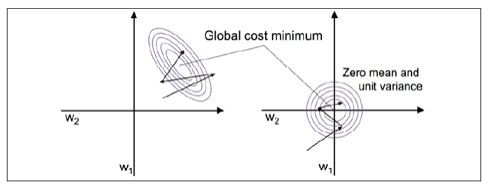
\includegraphics[scale=1]{../05-pictures/lesson-2-1_pic_4.png}
	\end{center}
\end{frame}
%
%..................................................................
%
\begin{frame}{Introduction}{Data Pre-Processing}
\begin{itemize}
\item
\end{itemize}
\end{frame}
%
%..................................................................
%
\begin{frame}{Introduction}{Data Pre-Processing}
\begin{itemize}
\item
\end{itemize}
\end{frame}
